\documentclass{article}
\usepackage{graphicx}
\usepackage{amsmath}
\usepackage{pgfplots}
\usepackage{physics}
\usepackage{cancel}
\usepackage{enumitem}
\usepackage{txfonts}

\pgfplotsset{compat=1.18}

\usepackage[a4paper, top=1cm, bottom=2cm, left=2cm, right=2cm, includehead, includefoot]{geometry}

\begin{document}

\noindent
Physics 4A - Classical Mechanics \hfill Prof. Roger King

\noindent\rule{\textwidth}{0.4pt}

\begin{center}
    \textbf{\LARGE Homework 3} \\
    \vspace{12pt}
    \large Aaron W. Tarajos \\
    \textit{\today}
\end{center}

\noindent\rule{\textwidth}{0.4pt}

\section*{Problem 1}
Is it possible to have $\left| \va A + \va B \right| = \left| \va A - \va B\right|$? If so, illustrate with a diagram.

\subsection*{Solution}
$\left| \va A + \va B \right| = \left| \va A - \va B\right|$ are equal when the magnitude of the respective sum vectors are equal to eachother.
The magnitude of the sum of two vectors, $\va A$ and $\va B$ is;

\[
\sqrt{|\va A|^2 + |\va B|^2 + 2|A|\ |B|\cos\theta}
\]
so we have

\begin{align*}
	\sqrt{|\va A|^2 + |\va B|^2 + 2|A|\ |B|\cos\theta} &= \sqrt{|\va A|^2 + |\va B|^2 - 2|\va A|\ |\va B|\cos\theta} \\
	|\va A|^2 + |\va B|^2 + 2|\va A|\ |\va B|\cos\theta &= |\va A|^2 + |\va B|^2 - 2|\va A|\ |\va B|\cos\theta \\
	|\va A|^2 + |\va B|^2 + 4|\va A|\ |\va B|\cos\theta &= |\va A|^2 + |\va B|^2 \\
	|\va A|^2 + 4|\va A|\ |\va B|\cos\theta &= |\va A|^2 \\
	4|\va A|\ |\va B|\cos\theta &= 0 \quad .
\end{align*}
We know that $\cos\theta=0$ when $\theta = 90^\circ$ which means that the magnitude of the sum and difference of two vectors $\va A$ and $\va B$ are equal when they are perpendicular to eachother.

\begin{figure}[ht!]
\centering
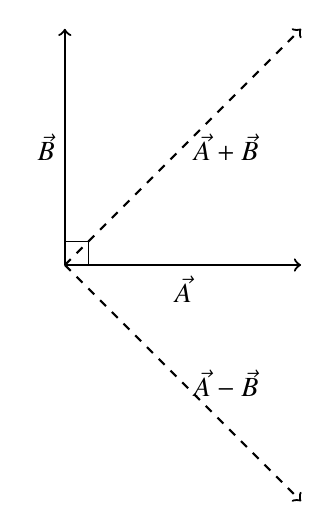
\begin{tikzpicture}[scale=1]
    % Draw vector A
    \draw[->, thick] (0,0) -- (3,0) node[midway, below] {$\vec{A}$};

    % Draw vector B (perpendicular to A)
    \draw[->, thick] (0,0) -- (0,3) node[midway, left] {$\vec{B}$};

    % Draw vector A+B
    \draw[->, thick, dashed] (0,0) -- (3,3) node[midway, right] {$\vec{A} + \vec{B}$};

    % Draw vector A-B
    \draw[->, thick, dashed] (0,0) -- (3,-3) node[midway, right] {$\vec{A} - \vec{B}$};

    % Mark the right angle
    \draw (0.3,0) -- (0.3,0.3) -- (0,0.3);

\end{tikzpicture}
\end{figure}

\newpage
\section*{Problem 2}
Four vectors, each of magnitude 2.50 m, are shown in the figure.
(a) Express each in unit vector notation.
(b) Express their sum in unit vector notation.
(c) What is the magnitude and direction of their sum?

\begin{figure}[ht]
    \centering
    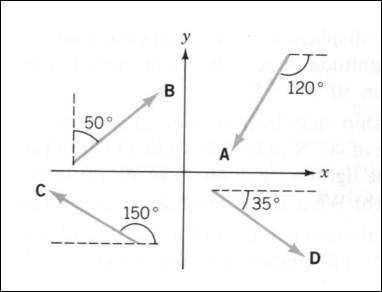
\includegraphics[scale=0.5]{graph-1.png}
\end{figure}

\subsection*{Solution}
\subsubsection*{Part a:}
Converting a vector from direction magnitude notation to unit vector notation starts by finding the component vectors of each vector.
We find the component vectors by finding the $\sin$ and $\cos$ of each vector given the angle.
The problem is that the reference angle is not exactly correct as given to just plug them into our trig functions and get the correct component vectors.
Therefore we have to use the given angle to find the correct angle $\theta$ for our trig functions.
For $\vb A$ the reference angle is drawn relative to the horizontal axis but drawn clockwise instead of counter clockwise, so we just have to use $-120^\circ$ instead.
\[
	a_y = 2.50\sin(-120) \quad \text{and} \quad a_x = 2.50\cos(-120)
\]
Then we multiply the result by the respective unit vector
\[
	\vb A = -1.25 \vu i + -2.165 \vu j
\]
$\vb D$ has effectively the same issue as $\vb A$, so we change the sign of the reference angle.
\[
	\vb D = 2.5\cos(-35) + 2.5\sin(-35)
\]
\[
	\vb D = 2.048 \vu i + -1.434 \vu j
\]
$\vb B$ is relative to a line parallel to the $y$-xis and so we take $90^\circ - 50^\circ = 40^\circ$ and use that for $\theta$.
\[
	\vb B = 2.5\cos(40) + 2.5\sin(40)
\]
\[
	\vb B = 1.915 \vu i + 1.607 \vu j
\]
Then $\vb C$ is already drawn relative to a line parallel to the $x$-axis in the correct direction so we simply use the angle as is.
\[
	\vb C = 2.5\cos(150) + 2.5\sin(150)
\]
\[
	\vb C = -2.165 \vu i + 1.25\vu j
\]

\subsubsection*{Part b:}
The sum in unit vector notation is simply the sum of each component;
\[
	\vb S = -1.25 \vu i + 2.048 \vu i + 1.915 \vu i -2.165 \vu i -2.165 \vu j -1.434 \vu j + 1.607 \vu j + 1.25\vu j
\]
and then combine like terms
\[
	\vb S = 0.548 \vu i + -0.742 \vu j
\]

\subsubsection*{Part c:}
We convert unit vector notation to magnitude direction notation by finding the length of the line connecting to two unit vectors and the direction by $\arctan (s_y/s_x)$.
\[
	\sqrt{\left(0.548\right)^2 + \left(-0.742\right)^2} = 0.922\ \text{m}
\]
and

\[
	\arctan \frac{-0.742}{0.548} = 306.6^\circ
\]
We know the degrees are correct because the input is within the restricted domain of $\arctan$ of $(-\pi/ 2, \pi/2)$.

\section*{Problem 3}
An object follows as shown below. What is the displacement from the last point to the
starting point? Express your answer (a) in unit vector notation, and (b) as a magnitude and
direction.

\begin{figure}[ht]
    \centering
    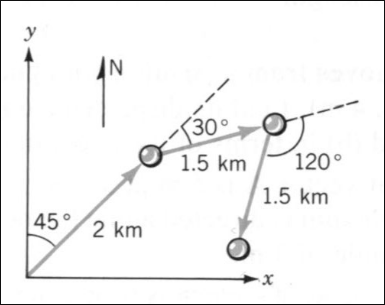
\includegraphics[scale=0.5]{graph-2.png}
\end{figure}

\subsection*{Solution}
\subsubsection*{Part a:}
We need to convert each vector into unit vector notation and then take the sum. The magnitudes are given but we have to find $\theta$ for each vector from the given reference angles.
\begin{align*}
	\vb |A| = 2\ \text{km} &\quad \theta_A = 90 - 45 = 45^\circ \\
	\vb |B| = 1.5\ \text{km} &\quad \theta_B = 90 - 45 - 30 = 15^\circ \\
	\vb |C| = 1.5\ \text{km} &\quad \theta_C = 90 - 45 - 30 - 120 = -105^\circ \\
\end{align*}
Finding sin and cos for each vector given the angles we obtain
\begin{align*}
	\vb A = 2\cos (45) + 2\sin (45) &= 1.414 \vu i + 1.414 \vu j \\
	\vb B = 1.5\cos (15) + 1.5\sin (15) &= 1.449 \vu i + 0.388 \vu j \\
	\vb C = 1.5\cos (-105) + 1.5\cos (-105) &= -0.388 \vu i + -1.449 \vu j
\end{align*}
adding these unit vectors together we obtain the displacement in vector unit notation as;
\[
	\vb S = 2.475 \vu i + 0.353 \vu j
\]

\subsubsection*{Part b:}
To convert the sum vector in unit notation to magnitude direction notation, we find the length of the side connecting the two scaled unit vectors and the arctangent angle subtended by them.
\[
	|S| = \sqrt{(2.475)^2 + (0.353)^2} = 2.50\ \text{km}
\]
\[
	\theta = \arctan \frac{0.353}{2.475} = 8.117^\circ
\]

\section*{Problem 4}
Given two vectors, $\va A  = 5.00 \vu i + 2.00 \vu j$, and $\va B = -2.00 \vu i - 3.00 \vu j$, find
(a) $\va A + \va B$
(b) $\left|\va A + \va B\right|$
(c) $\left|\va A - \va B\right|$
(d) $A - B$

\subsection*{solution}
\subsubsection*{Part a:}
We simply sum the respective unit vectors
\[
	\va S = 5.00 \vu i - 2.00 \vu i + 2.00 \vu j - 3.00 \vu j = 3.00 \vu i - 1.00 \vu j
\]
\subsubsection*{Part b:}
We find the magnitude as the length of the side connecting the two scaled unit vectors
\[
	\left|\va S\right| = \sqrt{(3.00)^2 + (-1.00)^2} = 3.162
\]

\subsubsection*{Part c:}
We find the magnitude of subtracting $\va B$ from $\va A$ by first switching the direction of the unit vectors of $\va B$ and then take the sum of the respective unit vectors.
\[
	\va S^\prime = 5.00 \vu i + 2.00 \vu i + 2.00 \vu j + 3.00 \vu j = 7.00 \vu i + 5.00 \vu j
\]
Then the magnitude is solved the same as before;
\[
	\left|\va S^\prime\right| = \sqrt{7^2 + 5^2} = 8.602
\]

\subsubsection*{Part d:}
We find the difference in the magnitude of $\va A$ and $\va B$ by
\[
	A = \sqrt{5^2 + 2^2} = 5.385
\]
and
\[
	B = \sqrt{(-2)^2 + (-3)^2} = 3.606
\]
and the difference then is
\[
	5.385 - 3.605 = 1.78
\]

\section*{Problem 5}
Find the components of the following vectors: (a) $\va P$ of length 5.50 m directed at $160^\circ$
counterclockwise from the $+x$ axis; (b) $\va Q$ of length 3.50 m directed at $120^\circ$ clockwise from the
$+y$ axis.

\subsection*{Solution}
\subsubsection*{Part a:}
Counter clockwise from the $+x$ axis is the correct orientation to use our angle as is for our trig functions. Therefore;
\begin{align*}
	\va P &= (p_x,p_y)\\
	&= (5.5\cos(160),5.5\sin(160)) \\
	&= (-5.168,1.881)
\end{align*}

\subsubsection*{Part b:}
Given that the $+y$ axis is $90^\circ$ from the $+x$ axis and we are rotating $120^\circ$ clockwise we can subtract $120^\circ$ from $90^\circ$ to give our position relative to the $+x$ axis as $-30^\circ$ and then evaluate the components as normal;
\begin{align*}
	\va Q &= (q_x,q_y)\\
	&= (3.5\cos(-30),3.5\sin(-30)) \\
	&= (1.75,-3.03)
\end{align*}

\section*{Problem 6}
Two vectors have equal magnitudes of 2.0 m. Find graphically the angle between them if the
magnitude of their resultant is (a) 3.0 m; (b) 1.0 m. In each case use the law of cosines to confirm
your answer.

\subsection*{Solution}
We can start by drawing a line of edge length 3 and two lines of edge length 2 and then arrange them such that all the lines form a triangle. Upon doing that we measure the angle formed by the two edges of length 2 with a protractor and find the angle is approximately $95^\circ$. Doing the same for edge length 1, we find that the angle is apprixmately $28^\circ$.
\begin{figure}[ht]
    \centering
    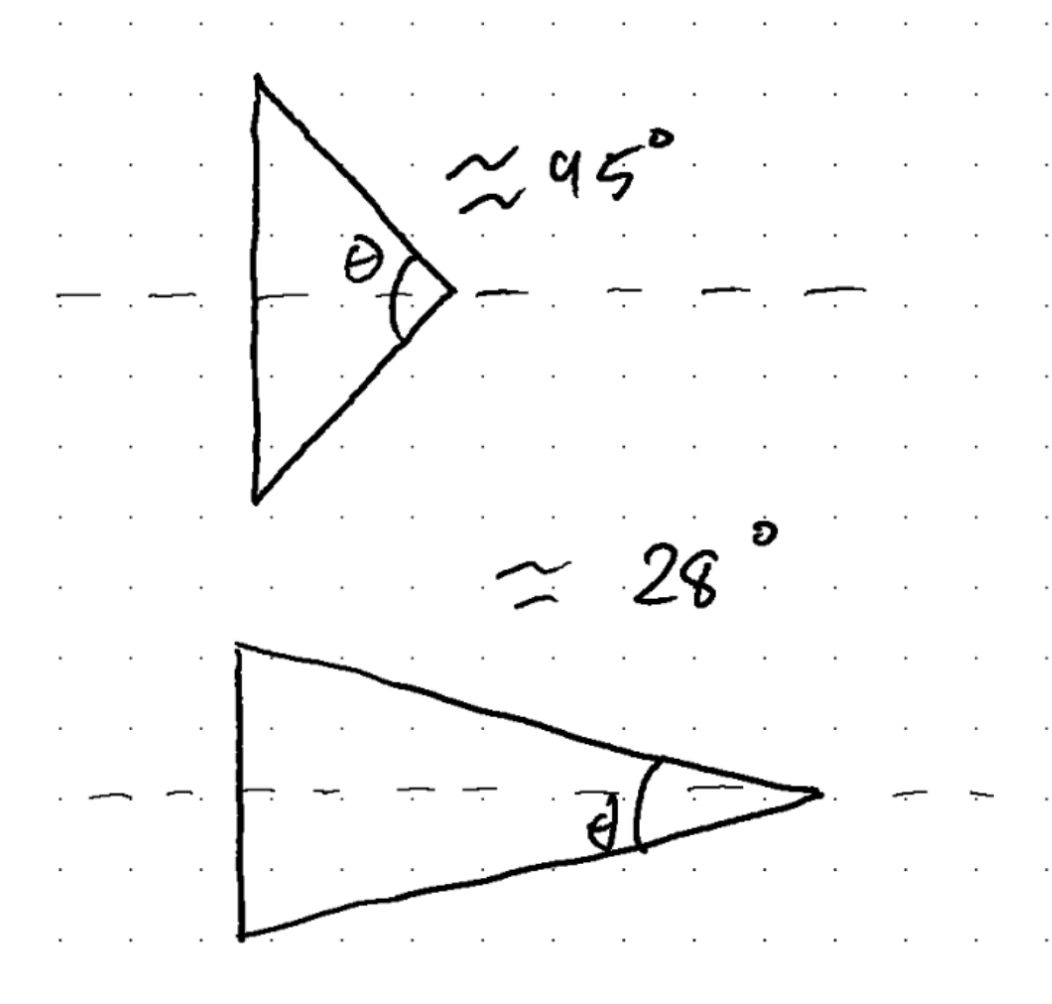
\includegraphics[scale=0.20]{drawing.png}
\end{figure}

Using the law of cosines we know that

\[
	C = \sqrt{A^2 + B^2 - 2AB \cos\theta}
\]
and so we can solve for both of the given resultants by isolating $\cos\theta$
\begin{align*}
	C^2 &=  A^2 + B^2 - 2AB \cos\theta \\
	\cos\theta &= \frac{A^2 + B^2 - C^2}{2AB} \\
	\theta &= \cos^{-1}\left( \frac{A^2 + B^2 - C^2}{2AB} \right)
\end{align*}
plugging in our given values for the resultants;
\[
	\theta_1 = \cos^{-1}\left( \frac{2^2 + 2^2 - 3^2}{2 (2) (2)} \right) = 97.181^\circ
\]
\[
	\theta_2 = \cos^{-1}\left( \frac{2^2 + 2^2 - 1^2}{2 (2) (2)} \right) = 28.955^\circ
\]

\section*{Problem 7}
An airplane is flown in the direction $30^\circ$ W of N. If the magnitude of the westerly component
of the displacement is 100. km, how far north does it travel?

\subsection*{Solution}
We are effectively given

\[
	l \cdot \cos(120) = 100\ \text{km}
\]
where $l$ is the scalar for the base vector given by $\cos (120)$. Therefore, we solve for $l$ and then use it to find the northern component.
\[
	l = \frac{100}{\cos(120)} = 200
\]
Then the northern component is given by
\[
	N = 200 \sin(120) = 173.205\ \text{km}
\]

\section*{Problem 8}
A rectangular coordinate system with axes $x^\prime$ and $y^\prime$ is rotated by angle $\theta$ from axes $x$ and $y$
as shown in the figure. (a) What are the components of the position vector $\vb r$ in the two
coordinate systems? (b) Use the results of part (a) to shown that the coordinates of a point $\vb P$ in
the two systems are related by
\[
	x^\prime = x\cos(\theta) + y\sin(\theta)
\]
\[
	y^\prime = -x\sin(\theta) + y\cos(\theta)
\]

\begin{figure}[ht]
    \centering
    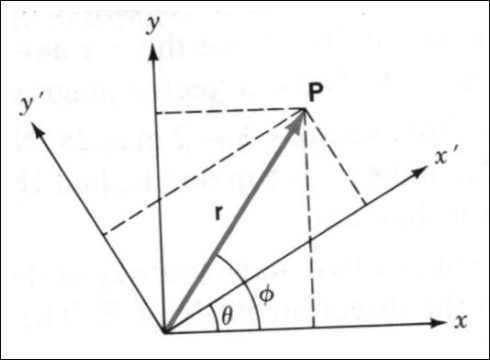
\includegraphics[scale=0.5]{graph-3.png}
\end{figure}

\subsection*{Solution}
\subsubsection*{Part a:}
Let $\vb r$ be the vector in reference to the $x$ and $y$ coordinate system, and $\vb r^\prime$ be the vector in reference to the $x^\prime$ and $y^\prime$ system. Then,
\[
	\vb r^\prime = |\vb r| \cos (\phi - \theta) + |\vb r| \sin(\phi - \theta)
\]
and
\[
	\vb r = |\vb r| \cos \phi + |\vb r| \sin \phi
\]
\subsubsection*{Part b:}
If the coordinates of $P$ are represented by $(x,y)$ and $(x^\prime,y^\prime)$ in their respective coordinate systems. The relationship between the point in these two coordinate systems are related by
\[
	x^\prime = x\cos(\theta) + y\sin(\theta)
\]
\[
	y^\prime = -x\sin(\theta) + y\cos(\theta)
\]
Proof:\\
Let $\vb r^\prime$ be the vector from the origin to the point $P$ in the $(x^\prime, y^\prime)$ coordinate system where;
\begin{align*}
	\vb r^\prime &= |\vb r| \cos (\phi - \theta) + |\vb r| \sin(\phi - \theta) \\
		     &= |\vb r| \cos\phi \cos\theta + |\vb r| \sin\phi \sin\theta + |\vb r| \sin\phi \sin\theta - |\vb r| \cos\phi \cos\theta
\end{align*}
because we know the $x$ component and $y$ component of $\vb r$ are $|\vb r|\cos\phi$ and $|\vb r|\sin\phi$ respectively we can replace those terms in our vector $\vb r^\prime$ to obtain the result;
\[
	\vb r^\prime = \left( x\cos\theta + y\sin\theta \right) + \left( -x\sin\theta + y\cos\theta \right) \quad \blacksquare
\]

\end{document}
